
\documentclass{bredelebeamer}
\usepackage{tikz}


%%%%%%%%%%%%%%%%%%%%%%%%%%%%%%%%%%%%%%%%%%%%%%%%



\title[]{Smith-Waterman Algorithm for Pairwise Local Alignment}


\author[ Kawshik, Imon and Maisha]{Kawshik Kumar Paul(1705043) \linebreak Monirul Haque Imon(1705054) \linebreak Maisha Rahman Mim (1705060)}

% La commande \inst{...} Permet d'afficher l' affiliation de l'intervenant.
% Si il y a plusieurs intervenants: Marcel Dupont\inst{1}, Roger Durand\inst{2}
% Il suffit alors d'ajouter un autre institut sur le modèle ci-dessous.

\titlegraphic{
\includegraphics[height=1.5cm]{buetlogo}}
\institute[BUET]{Department of Computer Science and Engineering \\ Bangladesh University of Engieering and Technology \\ Dhaka, Bangladesh }



\date{\today}
% Optionnel. La date, généralement celle du jour de la conférence

\subject{Sujet de votre diaporama}
% C'est utilisé dans les métadonnes du PDF



\logo{

\includegraphics[scale=0.15]{buetlogo.png}
}



%%%%%%%%%%%%%%%%%%%%%%%%%%%%%%%%%%%%%%%%%%%%%%%%%%%%%%%%%%%%%%%%%%%%%
\begin{document}

\begin{frame}
  \titlepage
\end{frame}





\begin{frame}{Lecture Outline}
  \tableofcontents
  % possibilité d'ajouter l'option [pausesections]
\end{frame}




\section{Sequence Alignment}

\begin{frame}{Sequence Alignment}
\large{
\begin{itemize}
    \item Why do we need to align sequence?
    \item Evolutionary Relationships
\end{itemize}
}
\end{frame}
\subsection{Why do we need to align sequence?}
\begin{frame}{Why do we need to align sequence?}
\begin{itemize}
\item Comparing DNA/protein sequences for
\begin{itemize}
    \item Similarity
    \item Homology
\end{itemize}

\item Prediction of function

\item Construction of phylogeny
 Shotgun assembly
\begin{itemize}
    \item  End-space-free alignment / overlap alignment
\end{itemize}
\item  Finding motifs
\end{itemize}
\end{frame}
\subsection{Definition}
\begin{frame}{Sequence Alignment}
\begin{itemize}
    \item  Procedure of comparing to (Pairwise) or more (Multiple) sequences by searching for a series of individual characters that are in the same order in the sequence.
\newline
\newline
\end{itemize}
\resizebox{\linewidth}{!}{
\begin{table}[scale=0.4\textwidth]
\begin{tabular}{cccccccccccccccccccc}
G & C & T & A & G & T & C & A & G & A & T & C & T & G & A & C & G & C & T & A \\
 &  & | &  & | & | & | & | &  & | & | & | & | & | & | & | & | & | &  &  \\
 &  & T & G & G & T & C & A & C & A & T & C & T & G & C & C & G & C &  & 
\end{tabular}
\end{table}}
   
\end{frame}
\section{Score Matrix}
\begin{frame}{Score Matrix}
   \begin{itemize}
       \item Instead of having a single match/mismatch 
score for every pair of nucleotides or amino 
acids, consider chemical, physical, 
evolutionary relationships:
\begin{itemize}
       \item  alanine vs. valine or alanine vs. lysine? Alanine and valine are both small and hydrophobic, but lysine is large and charged large and charged.
 \item  which substitutions occur more in nature?
   \end{itemize} 
   \item Assign scores to each pair of symbol
\begin{itemize}
 \item   Higher score means more similarity.
   \end{itemize} 
   \end{itemize} 
\end{frame}
\begin{frame}{Score Matrix}
\begin{itemize}
       \item DNA
\begin{itemize}
       \item  Match = +1
        \item  Mismatch = -3
         \item   Gap penalty = -5
          \item  Gap extension penalty = -2

   \end{itemize} 
   \item Protein sequences
\begin{itemize}
 \item Blossum62 matrix
         \item   Gap open penalty = -11
          \item  Gap extension penalty = -1
   \end{itemize} 
   \end{itemize}
\end{frame}
 \section{Dynamic Programming}
 \begin{frame}{}
    \large{
    \begin{itemize}
 \item How do we compute the best alignment?
   \end{itemize} 
   
    }  
 \end{frame}
  \begin{frame}{Alignment is additive}
   
    \begin{itemize}
 \item Observation:

 \par The score of aligning $x_1...x_M$ and $y_1...y_N$ is additive
 \newline 
\par
   Say that \quad $x_1...x_i$ \quad $x_{i+1}...x_M$ \linebreak \quad aligns to \quad $y_1...x_j$ \quad $x_{j+1}...x_N$
   \newline
    \newline
    The two scores add up:
    \quad
   $$F(x[1:M], y[1:N]) = F(x[1:i], y[1:j]) + F(x[i+1:M], y[j+1:N])$$
   
   \end{itemize} 
 \end{frame}
 \begin{frame}{Types of alignment}
    \begin{itemize}
 \item Global
          \begin{itemize}
     \item Strings of similar size
      \begin{itemize}
     \item Genes with a similar structure
     \item Larger regions with a preserved order (syntenic
regions)
   \end{itemize} 
   \end{itemize} 
   \item Local
    \begin{itemize}
     \item Finding similar regions among:
      \begin{itemize}
     \item Dissimilar regions
     \item Sequences of different lengths
   \end{itemize} 
   \end{itemize}
   \end{itemize}  
 \end{frame}
 \begin{frame}{}
     \begin{itemize}
         \item \large{Here we introduce Smith & Waterman Algorithm for local alignment...}
     \end{itemize} \end{frame}
  \begin{frame}{Dynamic Programming}
     \begin{itemize}
         \item Instead of evaluating every possible alignment, we can create a 
table of partial scores by breaking the alignment problem into subproblems.
\item Consider two sequences CACGA and CGA
\begin{itemize}
         \item we have three possibilities for the first position of the alignment
         \newline
% Please add the following required packages to your document preamble:
% \usepackage{multirow}
\begin{table}[]
\begin{tabular}{|c|c|c|}
\hline
First Position & Score               & Remaining seqs \\ \hline
C              & \multirow{2}{*}{+1} & ACGA           \\
C              &                     & GA             \\ \hline
--             & \multirow{2}{*}{-1} & CACGA          \\
C              &                     & GA             \\ \hline
C              & \multirow{2}{*}{-1} & ACGA           \\
--             &                     & CGA            \\ \hline
\end{tabular}
\end{table}
     \end{itemize}
     \end{itemize}
 \end{frame}
% \begin{columns}

% \begin{column}{0.5\textwidth}
% \begin{block}{Bloc simple}
% \begin{itemize}
% \item Premier point
% \end{itemize}
% \end{block}

% \begin{exampleblock}{Bloc exemple}
% \begin{itemize}
% \item Premier point
% \end{itemize}
% \end{exampleblock}

% \begin{alertblock}{Bloc alert}
% \begin{itemize}
% \item Premier point
% \end{itemize}
% \end{alertblock}

% \end{column}

% \begin{column}{0.5\textwidth}
% \boiteviolette{
% Une boite violette
% }

% \boiteorange{
% Une boite orange
% }

% \boitegrise{
% Une boite grise
% }



% \begin{tcolorbox}[tabvert,tabularx={X||Y|Y|Y|Y||Y}, boxrule=0.5pt, title=Mon tableau des prix]
% Couleur & Prix 1  & Prix 2  & Prix 3 \\\hline\hline
% Rouge   & 10.00   & 20.00   &  30.00 \\\hline
% Vert    & 20.00   & 30.00   &  40.00  \\\hline
% Bleu    & 30.00   & 40.00   &  50.00 \\\hline\hline
% Orange  & 60.00   & 90.00   & 120.00 
% \end{tcolorbox}

% \end{column}

% \end{columns}





\section{Les blocs}

\begin{frame}{Les blocs}

\begin{block}{Bloc simple}
\begin{itemize}
\item Premier point
\item Second point
\item Troisième point
\end{itemize}
\end{block}

\begin{exampleblock}{Bloc exemple}
\begin{itemize}
\item Premier point
\item Second point
\item Troisième point
\end{itemize}
\end{exampleblock}

\begin{alertblock}{Bloc alert}
\begin{itemize}
\item Premier point
\item Second point
\item Troisième point
\end{itemize}
\end{alertblock}
\end{frame}


\section{Les bo\^ites}

\begin{frame}{Les boites}

\begin{columns}

\begin{column}{0.5\textwidth}
\boitejaune{
Ceci est \\
une boite jaune
}

\boiteorange{
Ceci est \\
une boite orange
}

\boitemarron{
Ceci est \\
une boite marron
}
\end{column}

\begin{column}{0.5\textwidth}
\boiteviolette{
Ceci est \\
une boite violette
}

\boitebleue{
Ceci est \\
une boite bleue
}

\boitegrise{
Ceci est \\
une boite grise
}

\end{column}

\end{columns}


\end{frame}



\section{Les listes}
	\subsection{Liste à item}

\begin{frame}{Titre de la frame}

	\begin{itemize}
		\item premier élément de liste,
		\item deuxième élément de liste,
		\item troisième élément de liste.
	\end{itemize}
\end{frame} 

		\subsection{Liste énumérative} 
\begin{frame}{Titre de la frame} 
	\begin{enumerate}
		\item élément de liste numéro 1,
		\item élément de liste numéro 2,
		\item élément de liste numéro 3.  
	\end{enumerate}
\end{frame}


		\subsection{Liste descriptive} 
\begin{frame}{Titre de la frame} 
	\begin{description}
		\item [Thème de présentation : ] ces thèmes sont en fait...
		\item [Thème de couleur : ] gère tout ce qui est couleur...
		\item [Thème de police : ] s'occupe de tout ce qui est police, gras...
		\item [Thème interne : ] s'occupe de l'apparence des éléments...
	\end{description}
\end{frame}



\section{Le texte}

\begin{frame}{Titre de la frame} 

Voici du texte normal

\alert{Voici du texte \texttt{alert}}

\exemple{Voici du texte \texttt{exemple}}

\emph{Voici du texte \texttt{emphase}}

\end{frame}


\section{Les tableaux}

\begin{frame}{Tableaux}

% merci: http://tex.stackexchange.com/questions/112343/beautiful-table-samples

\begin{tcolorbox}[tabjaune,tabularx={X||Y|Y|Y|Y||Y}, boxrule=0.5pt]
Couleur & Prix 1  & Prix 2  & Prix 3   & Prix 4   & Prix 5 \\\hline\hline
Rouge   & 10.00   & 20.00   &  30.00   &  40.00   & 100.00 \\\hline
Vert    & 20.00   & 30.00   &  40.00   &  50.00   & 140.00 \\\hline
Bleu    & 30.00   & 40.00   &  50.00   &  60.00   & 180.00 \\\hline\hline
Orange  & 60.00   & 90.00   & 120.00   & 150.00   & 420.00
\end{tcolorbox}

\begin{tcolorbox}[tabvert,tabularx={X||Y|Y|Y|Y||Y}, boxrule=0.5pt, title=Mon tableau des prix]
Couleur & Prix 1  & Prix 2  & Prix 3   & Prix 4   & Prix 5 \\\hline\hline
Rouge   & 10.00   & 20.00   &  30.00   &  40.00   & 100.00 \\\hline
Vert    & 20.00   & 30.00   &  40.00   &  50.00   & 140.00 \\\hline
Bleu    & 30.00   & 40.00   &  50.00   &  60.00   & 180.00 \\\hline\hline
Orange  & 60.00   & 90.00   & 120.00   & 150.00   & 420.00
\end{tcolorbox}

\end{frame}


\begin{frame}{Tableaux}

% merci: http://tex.stackexchange.com/questions/112343/beautiful-table-samples

\begin{tcolorbox}[tabgris,tabularx={X||Y|Y|Y|Y||Y}, boxrule=0.5pt]
Couleur & Prix 1  & Prix 2  & Prix 3   & Prix 4   & Prix 5 \\\hline\hline
Rouge   & 10.00   & 20.00   &  30.00   &  40.00   & 100.00 \\\hline
Vert    & 20.00   & 30.00   &  40.00   &  50.00   & 140.00 \\\hline
Bleu    & 30.00   & 40.00   &  50.00   &  60.00   & 180.00 \\\hline\hline
Orange  & 60.00   & 90.00   & 120.00   & 150.00   & 420.00
\end{tcolorbox}

\begin{tcolorbox}[taborange,tabularx={X||Y|Y|Y|Y||Y}, boxrule=0.5pt, title=Mon tableau des prix]
Couleur & Prix 1  & Prix 2  & Prix 3   & Prix 4   & Prix 5 \\\hline\hline
Rouge   & 10.00   & 20.00   &  30.00   &  40.00   & 100.00 \\\hline
Vert    & 20.00   & 30.00   &  40.00   &  50.00   & 140.00 \\\hline
Bleu    & 30.00   & 40.00   &  50.00   &  60.00   & 180.00 \\\hline\hline
Orange  & 60.00   & 90.00   & 120.00   & 150.00   & 420.00
\end{tcolorbox}

\end{frame}



\section{Les images}

\begin{frame}{Titre de la frame} 

\begin{figure}
\centering
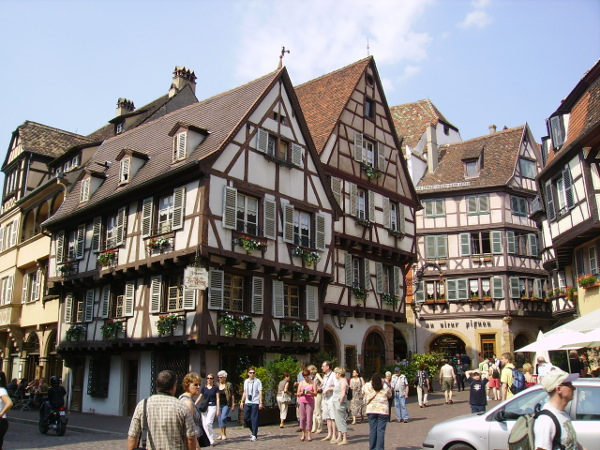
\includegraphics[scale=0.5]{images/architecturebretonne_wikipedia.jpg}
\caption{Éléments d'architecture bretonne typique du Sud de la France. (\href{http://commons.wikimedia.org/wiki/File:Colmar_-_Alsace.jpg}{Wikipédia.fr} CC-By-Sa)}
\end{figure}

\end{frame}



\end{document}
